\par Backgrounds are categorized into 3 classes that are defined according to the 
source of the $\tauvis$.   
If the \tauvis\ is reconstructed from a $\tau$ lepton, it is referred to as a {\it true} 
$\tauvis$. Treatment of this category has been briefly discussed in Section~\ref{sec:evSelCh} and 
is discussed in more detail in Section~\ref{sec:truetau}. Events in which a $\tauvis$ is reconstructed from an electron or muon  
constitute the $l\to\tau$ background. More on this in Section~\ref{sec:lepToTau}.
Events in which a $\tauvis$ is reconstructed from a jet, be it from a quark or gluon, 
constitute the $j\to\tau$ background. More on this in Section~\ref{sec:jetToTau}. 
The $j\to\tau$ and $l\to\tau$ backgrounds are collectively 
referred to here as the {\it Mis-ID}\footnote{For `misidentified $\tau$'.}  backgrounds. 

\subsection{Lepton to $\tau$}
\label{sec:lepToTau}
\par For the $l\to\tauvis$ backgrounds only the $e\to\tauvis$ contribution is estimated; 
the $\mu\to\tauvis$ background contamination in the signal region was found to be an order of magnitude smaller. 
Backgrounds in which a $\tauvis$ is matched in $\Delta R$ to an electron are 
applied a scale factor, which encodes the probability of an electron to fake a $\tauvis$. This 
scale factor is dependent on whether the reconstructed $\tauvis$ is 1-prong or 3-prong, so separate 
computations are performed. This scale factor was also observed to be dependent on $\eta$, so it was 
parametrized accordingly. 

\par To measure these scale factors the following $\Zee$ control region is designed 

\begin{enumerate}
\item exactly one electron matched to a single electron trigger;
\item exactly one medium \tauvis\ with charge opposite to the electron;
\item no $b-$tagged jets; and 
\item $\mT(e,\met)<40$~\GeV
\end{enumerate}  

Here, the electron is used as a tag, and the \tauvis\ as a probe. 
To ensure that the \tauvis\ and the electron originate from the \Zboson, the mass of the 
$e-\tauvis$ system is restricted to between 80~\GeV\ and 100~\GeV.

\par The scale factors were computed as the ratio of events that pass all selection criteria to those 
that pass all but not necessarily the presence of the \tauvis. This computation was 
performed in both data and simulation. In data, non-\Zee\ events were subtracted from data 
before the calculation was performed. Figure~\ref{fig:lepToTau} shows these scale factors, 
parametrized in $\eta$. They range from 0.5\% to 2.5\%.    

\begin{figure}[h]
\centering
   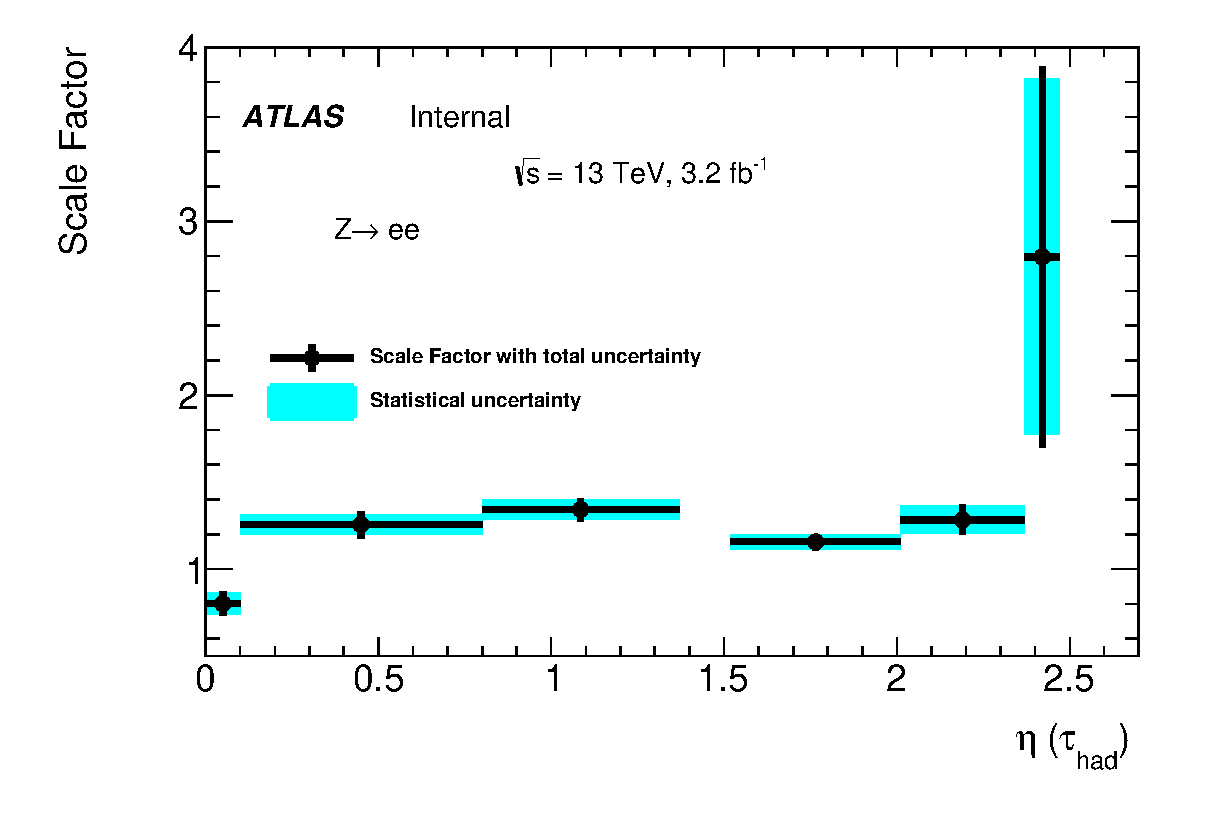
\includegraphics[width=0.8\textwidth]{figures/c7_evto_SF.eps}
\caption{Plot showing the probability of an electron to fake a \tauvis, parametrized in $\eta$}
\label{fig:lepToTau}
\end{figure}
 
\subsection{$j\to\tau$ backgrounds}
\label{sec:jetToTau}
\par The {\it Fake Factor Method (FFM)}, described in this section, is used to estimate $j\to\tau$ backgrounds. 
The strategy is to extrapolate to the signal region the number of events where a $\tauvis$ is reconstructed from a quark 
or gluon initiated jet, from a control region rich with quark or gluon initiated jets.
The extrapolation is handled by scale factors, referred to as {\it Fake Factors (\FF)}. 
During this extrapolation large uncertainties are accrued from differences between the said control region and 
the signal region. To minimize them, the control region is designed to be as close to the 
signal region as possible. The control region used here, referred to as 
the {\it anti-$\tau$} region, only differs from the signal region in that the reconstructed  
 \tauvis\ fails the identification criteria required in the signal region.  
More specifically, the anti-$\tau$ region is identical to the signal region except that its \tauvis\ is required 
to be not loose and its jet BDT score is required to be greater than 0.5.
Events in which a quark or gluon initiated jet fakes a $\tau$ lepton in the signal region, $N^\tau_{\text{fakes}}$.
are therefore estimated by weighting events in the anti-$\tau$ region, $N^{\text{anti-}\tau}_{\text{fakes}}$,
 with $\FF$ as summarized in Equation~\ref{eq:ffDef}. 

\begin{equation}
N^\tau_{\text{fakes}} = N^{\text{anti-}\tau}_{\text{fakes}}\times\FF
\label{eq:ffDef}
\end{equation}

\par The $\FF$ are measured from a region in data that is rich in quark or gluon initiated jets. This {\it 
measurement} control region must be different from the control region in which the $\FF$ are applied (e.g the 
one described in the preceding paragraph). It is however similar in the sense that the \tauvis\ is required 
to pass the same identification criteria. In this case it is required to be not loose and have 
a jet BDT score greater than 0.5. In that respect, it is referred to as the {\it anti-$\tau$-id}\footnote{To 
emphasize, this is not to be confused with the anti-$\tau$ region in which the \FF\ are applied.} region. 
A similar control region, but with the \tauvis\ required to pass the identification criteria that is 
demanded in the signal region, is also defined. This is called the $\tau-id$ control region.  
The number of events in the anti-$\tau$-id control region, $N_{\text{anti-}\tau\text{-id}}$, 
and the number of events in the $\tau-$id region, 
$N_{\tau-\text{id}}$, are extracted. The fake factors are then computed as 

\begin{equation}
\FF = \frac{N_{\tau-\text{id}}}{N_{\text{anti-}\tau\text{-id}}} 
\end{equation}

\subsubsection{Pre-validation}
\par To test the effectiveness of this method, fake factors from \ttbar\ simulation are applied 
on \ttbar\ events after a different selection criteria has been applied. 
Simulated \ttbar\ events with exactly one not loose $\tauvis$ make up the anti-$\tau$-id 
region. Similarly, events with exactly one medium $\tauvis$ make up the $\tau-$id region.
Since the probability of a jet being mis-identified as a $\tauvis$ depends on the jet substructure, \FF\ 
are parameterized in terms of parameters that describe the jet substructure. These are 
\begin{enumerate}
\item Transverse momentum of the \tauvis, $\pt^\tau$. This parameter is sensitive to the 
gluon or quark fractions in the jet;
\item $\tau$ decay mode. This is essentially a measure of the number of pions that the $\tau$ 
lepton decays to; and 
\item $b-$tagger weight. 
\end{enumerate}    

The \FF\ obtained in the \ttbar\ MC simulation are applied to \ttbar\ events that pass the 
preselection criteria defined in Table~\ref{tab:sigReg}. Figure~\ref{fig:ttClo} shows comparisons 
between estimation using \FF\ and direct MC estimation. 

\begin{figure}[h]
\begin{subfigure}{0.5\textwidth}
   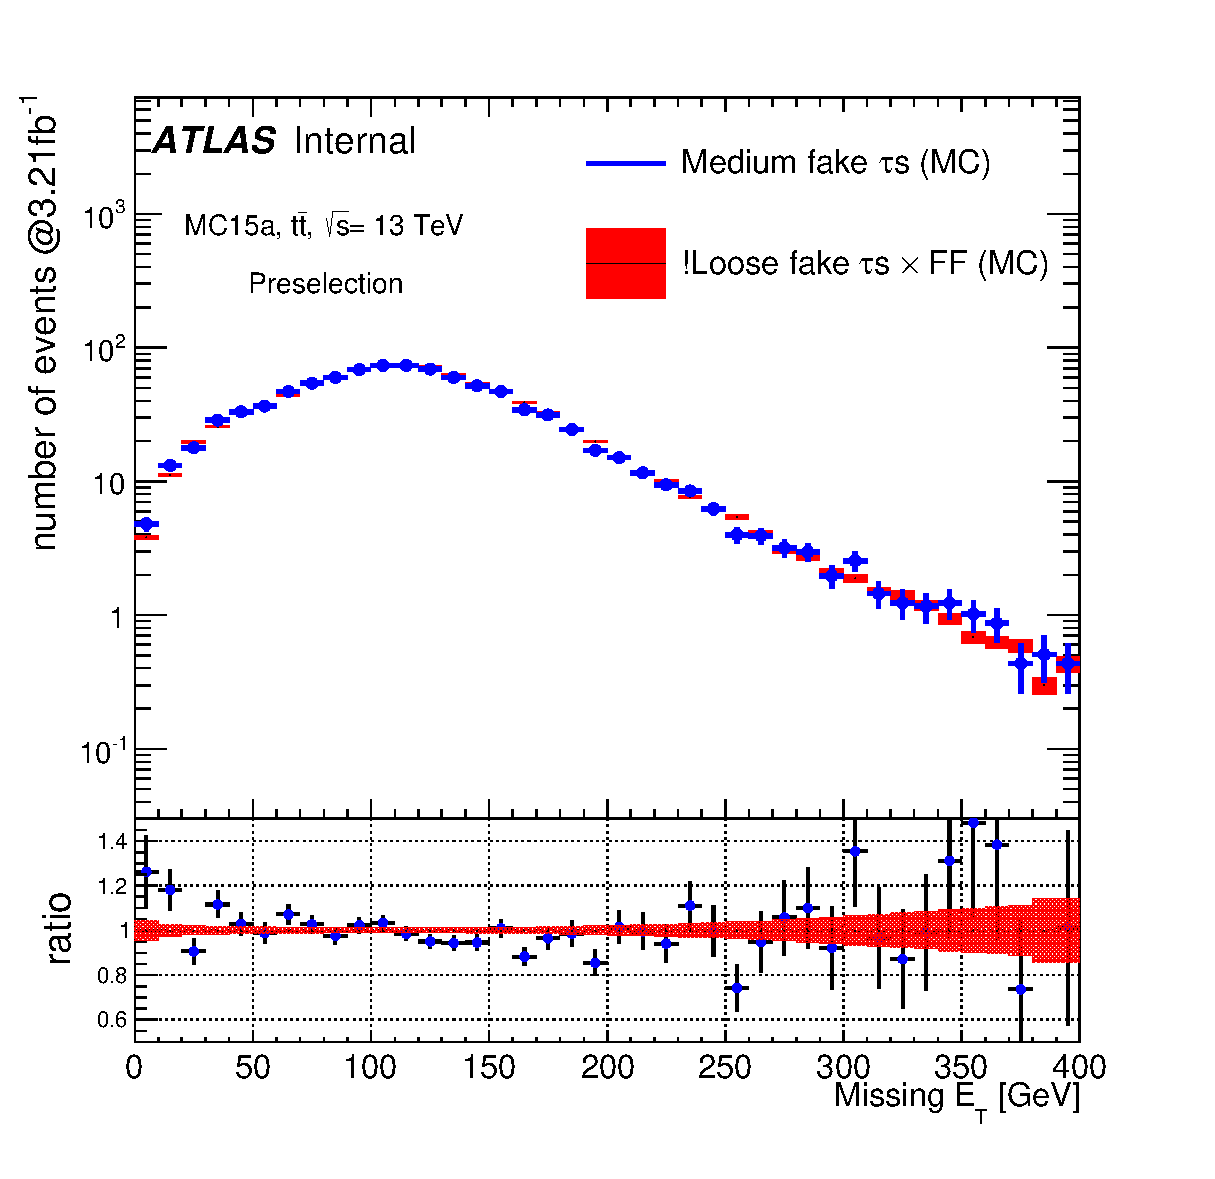
\includegraphics[width=\textwidth]{figures/Fake_MMClosure_met.eps}
\caption{\met\ in \ttbar closure region}
\end{subfigure} % 
\begin{subfigure}{0.5\textwidth}
   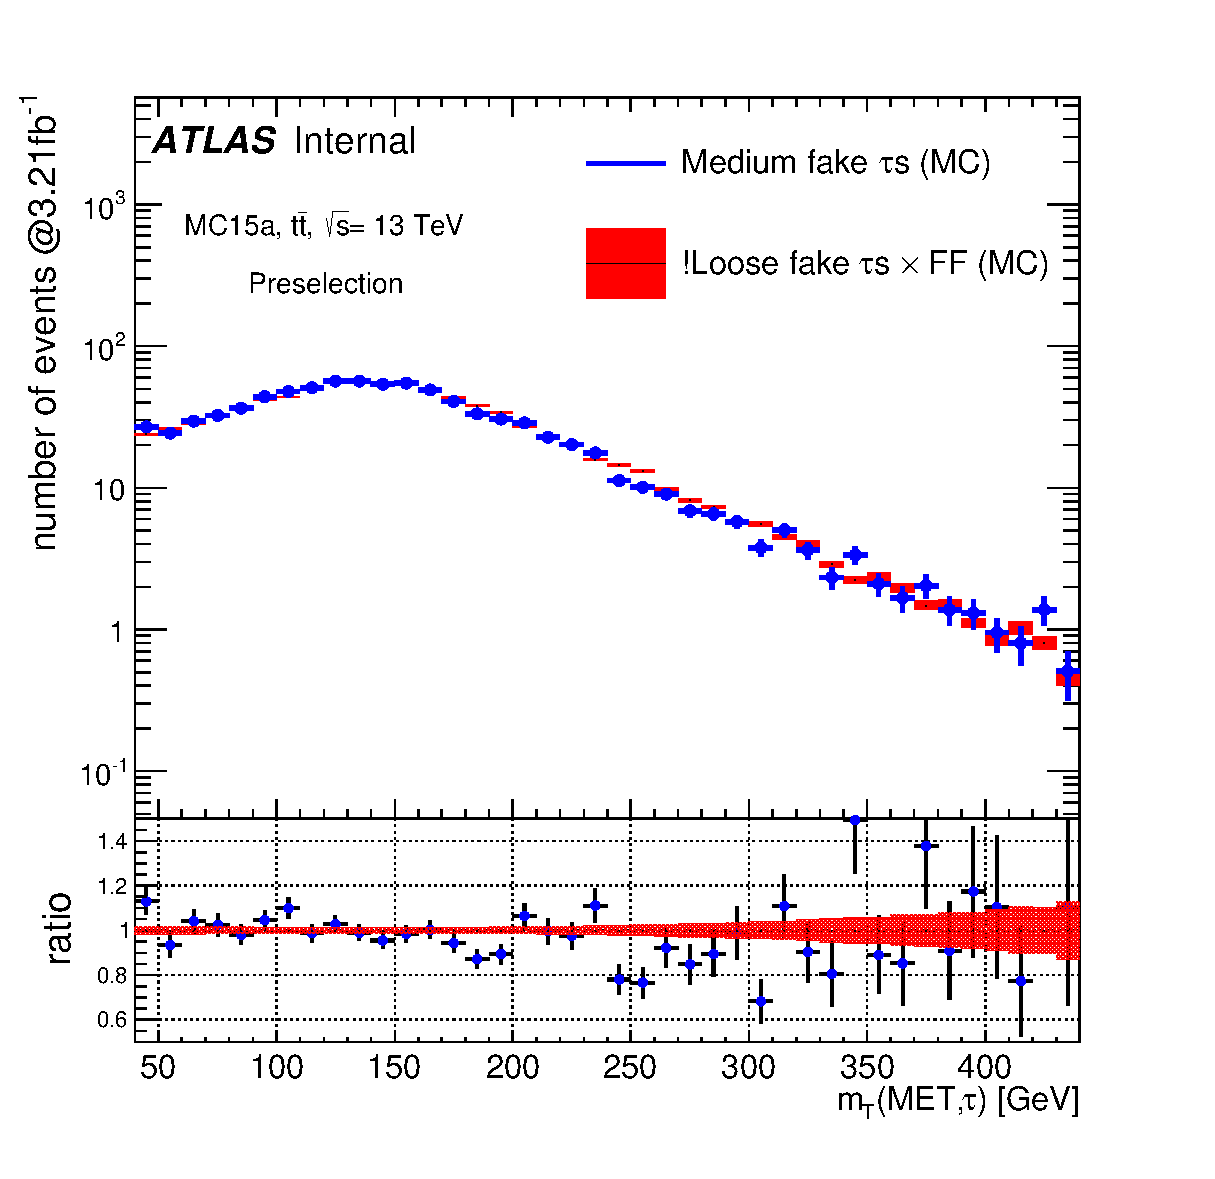
\includegraphics[width=\textwidth]{figures/Fake_MMClosure_MT.eps}
\caption{\mT\ in \ttbar closure region}
\end{subfigure}
\caption{Plots showing the comparison of estimations using direct MC versus the \FF\ method}
\label{fig:ttClo}
\end{figure}

\subsubsection{\FF\ measurement control regions}
\par Two regions in data that are rich in jets reconstructed as \tauvis\ are 
used to extract \FF. One of these regions is designed to be dominated by QCD multi-jet events,
 while the other is dominated by $\Wjets$ events. The former will be referred to as the {\it multi-jet} 
region while the latter as the $\Wjets$ region. The fraction of jets that are initiated by quarks 
in the multi-jet region is roughly the same as the fraction of jets that are initiated by gluons 
in the same region. In contrast, the \Wjets\ region is dominated by jets initiated by light-flavor quarks.
Since the substructure of jets is expected to depend on their source, it is necessary to evaluate the impact 
of these different sources on the final results. The multi-jet region is used as the nominal region for measuring 
\FF. Measurements taken from \Wjets\ are used as a systematic variation corresponding to the inclusion of a higher 
fraction of light-flavor quarks.  

\par The multi-jet region is similar to the signal region. It differs from the signal region 
in that it requires 0 $b-$tagged jets and $\met<80$~\GeV. Figure~\ref{fig:multiCR} shows 
\mT\ distributions for processes that pass this selection criteria. The \Wjets\ region is more different to the signal region than 
the multi-jet region. \met\ is required to be at most 150~\GeV, exactly one electron or muon must 
be present, no $b-$tagged jets, and $\mT(e/\mu,\met)>60$~\GeV. Figure~\ref{fig:wjetsFFcr} shows 
\mT\ distributions in this region.  

\begin{figure}[!h]
\begin{subfigure}{0.5\textwidth}
   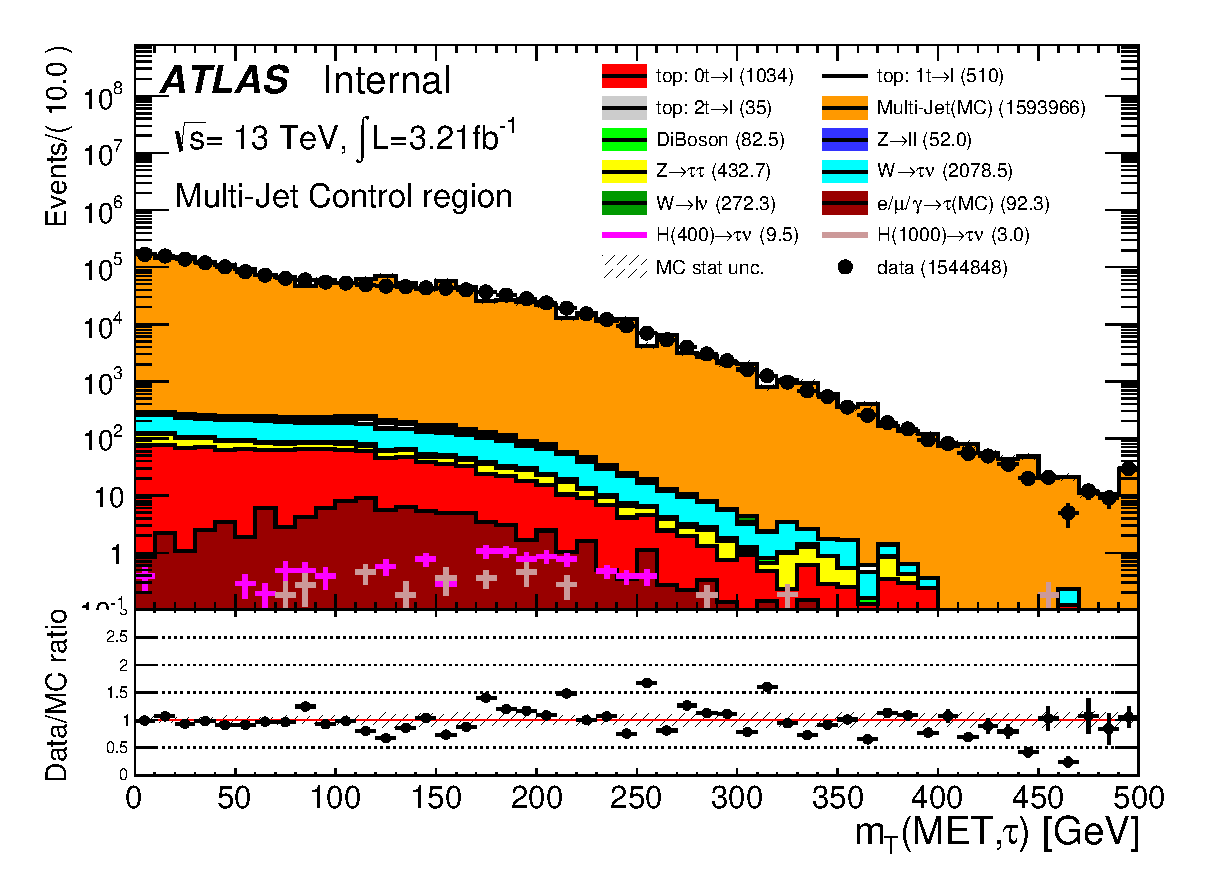
\includegraphics[width=\textwidth]{figures/data15_QCD_MT_log.eps}
\caption{Multi-jet region for \FF}
\label{fig:multiCR}
\end{subfigure} % 
\begin{subfigure}{0.5\textwidth}
   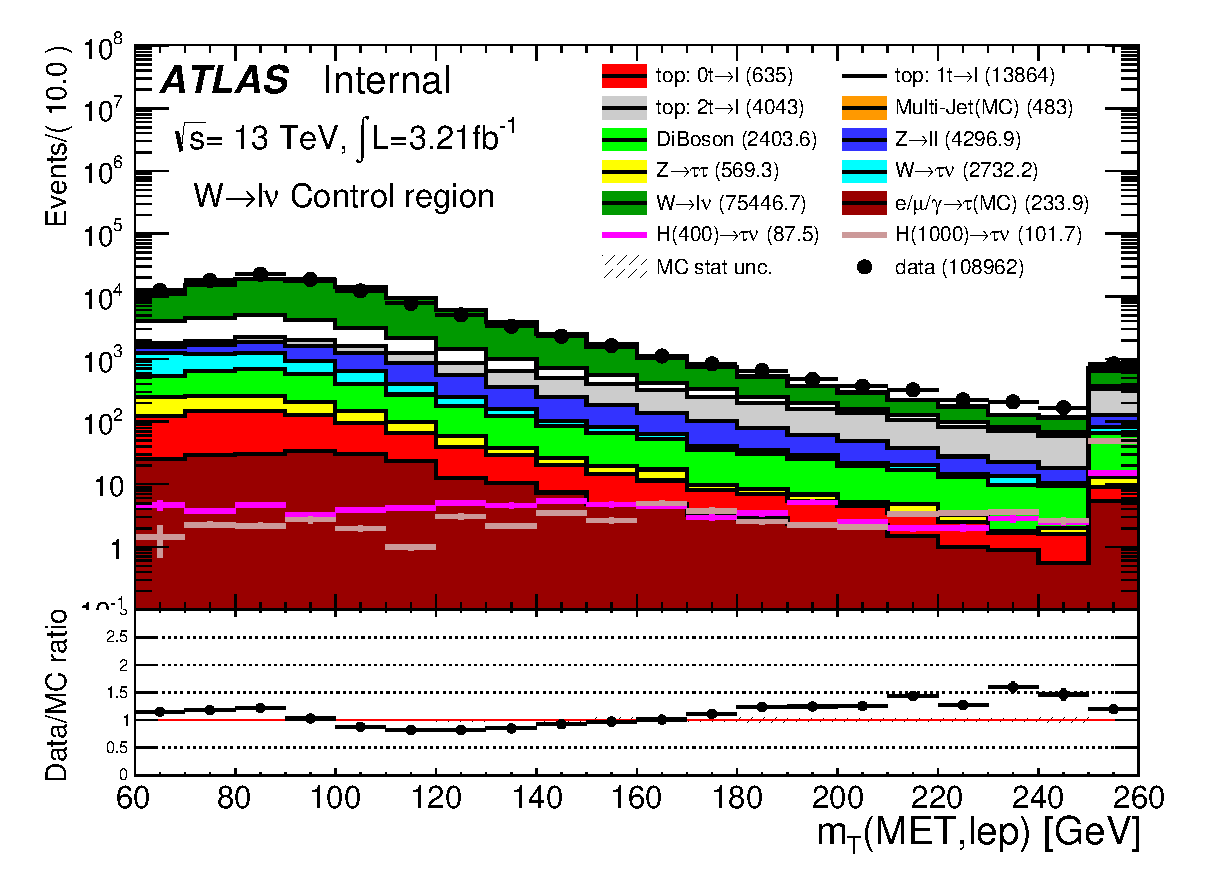
\includegraphics[width=\textwidth]{figures/data15_WCR_WlepMT_log.eps}
\caption{\Wjets\ region for \FF}
\label{fig:wjetsFFcr}
\end{subfigure}
\caption{Plots showing \mT\ distributions in the multi-jet and the \Wjets\ control regions}
\end{figure}

\par Figures~\ref{fig:ffA} and \ref{fig:ffB} show the \FF\ obtained from the multi-jet region. 
They are parametrized in $\pt$ computed separately for 1-prong and 3-prong $\tauvis$ candidates. 
Figure~\ref{fig:ffA} is from 2015 data while Figure~\ref{fig:ffB} is from 2016 data. The binning in 
\pt\ was optimized to have a minimal statistical uncertainty in each bin. For 2016 data the \FF\ dependence 
on the $b-$tag weight was insignificant so it wasnt pursued further.   

\begin{figure}[!h]
\begin{subfigure}{0.5\textwidth}
   \includegraphics[width=\textwidth]{figures/GetTauFFmed2D_2015.eps}
\caption{}
\label{fig:ffA}
\end{subfigure} % 
\begin{subfigure}{0.5\textwidth}
   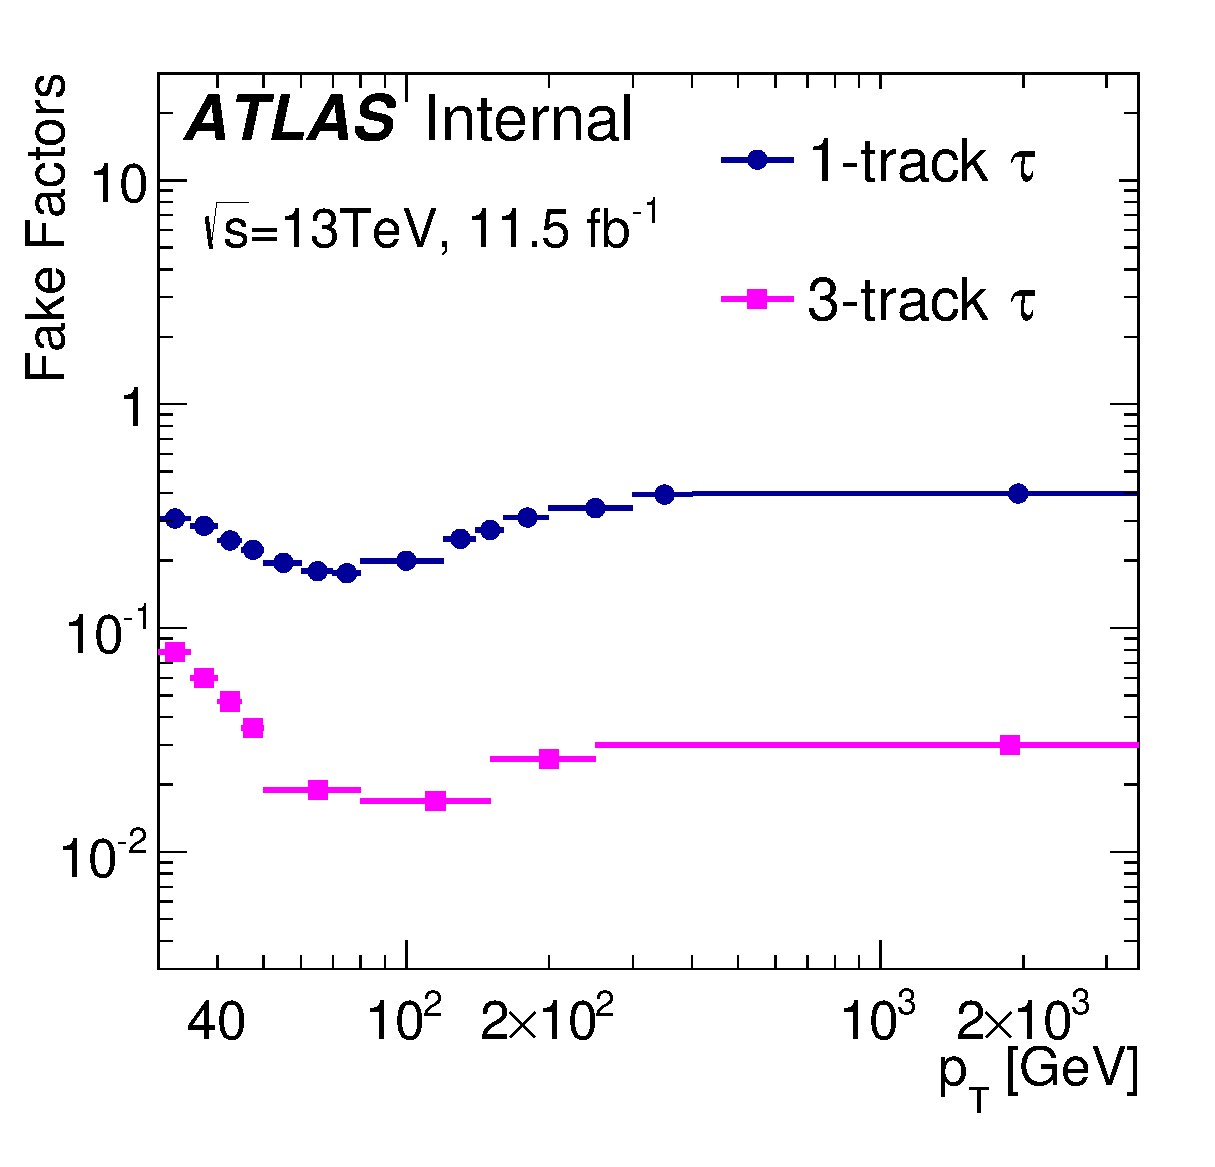
\includegraphics[width=\textwidth]{figures/GetTauFFmed2D_2016.eps}
\caption{}
\label{fig:ffB}
\end{subfigure}
\caption{Plots showing the measured \FF\ parametrized in \tauvis\ \pt}
\label{fig:ff}
\end{figure}

\subsubsection{Validation}
\par The \FF\ shown in Figure~\ref{fig:ff} were validated in several control regions. First is the 
multi-jet control region from which these \FF\ were measured. Figure~\ref{fig:clMultiJ} shows the 
estimated $j\to\tau$ contribution in this region, using the FFM. Overall, the estimation shows good 
\FF\ modelling in this region. 

\begin{figure}[h]
\begin{subfigure}{0.5\textwidth}
   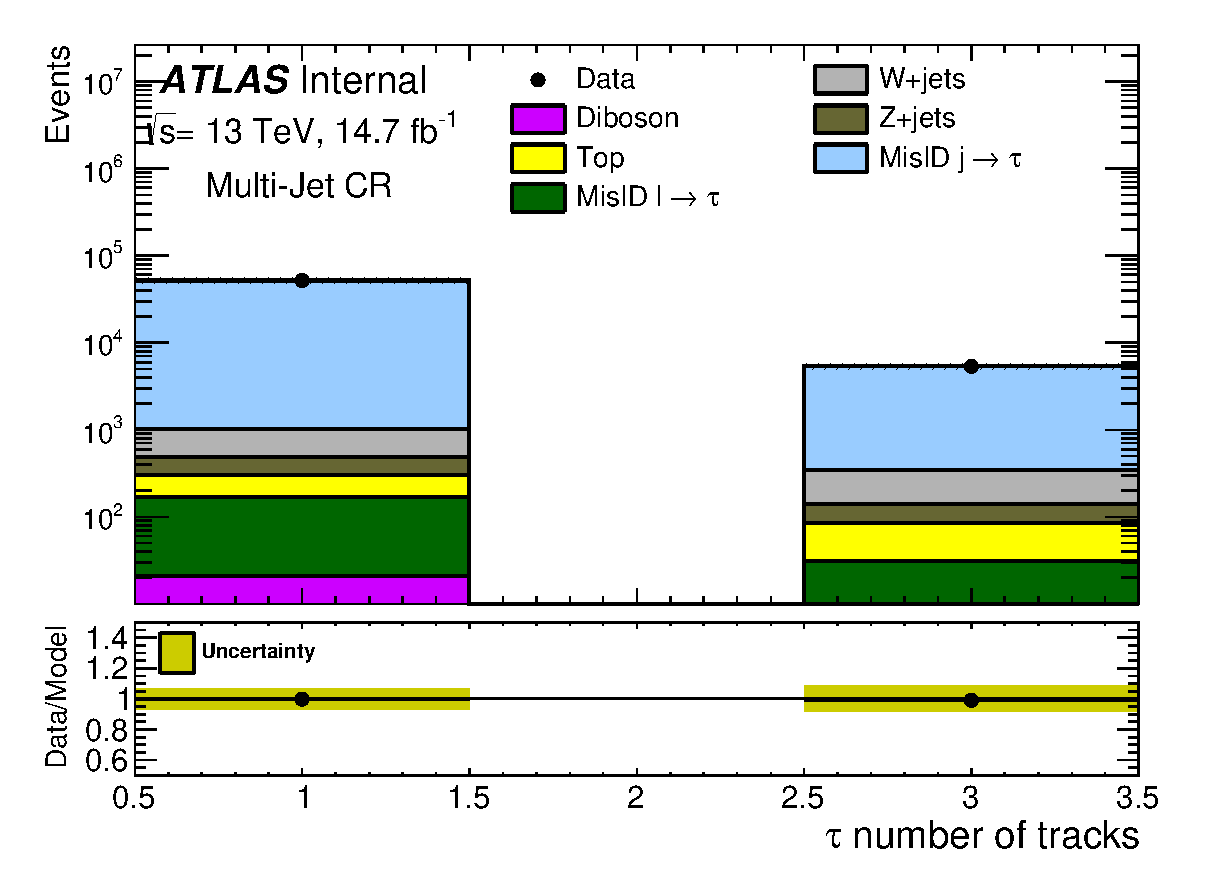
\includegraphics[width=\textwidth]{figures/DDQCD15_QCD_nTrack.eps}
\caption{}
\end{subfigure} % 
\begin{subfigure}{0.5\textwidth}
   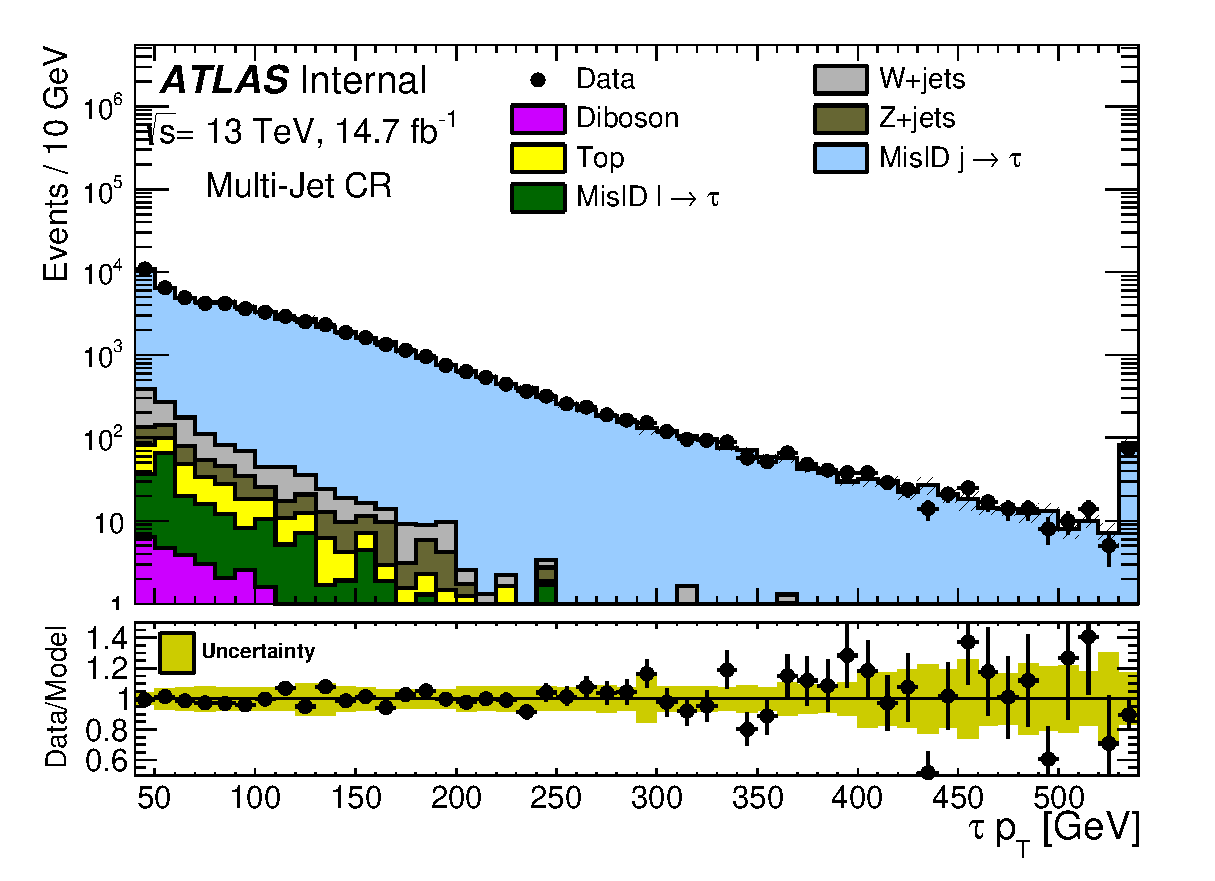
\includegraphics[width=\textwidth]{figures/DDQCD15_QCD_taupt_log.eps}
\caption{}
\end{subfigure}
\begin{subfigure}{0.5\textwidth}
   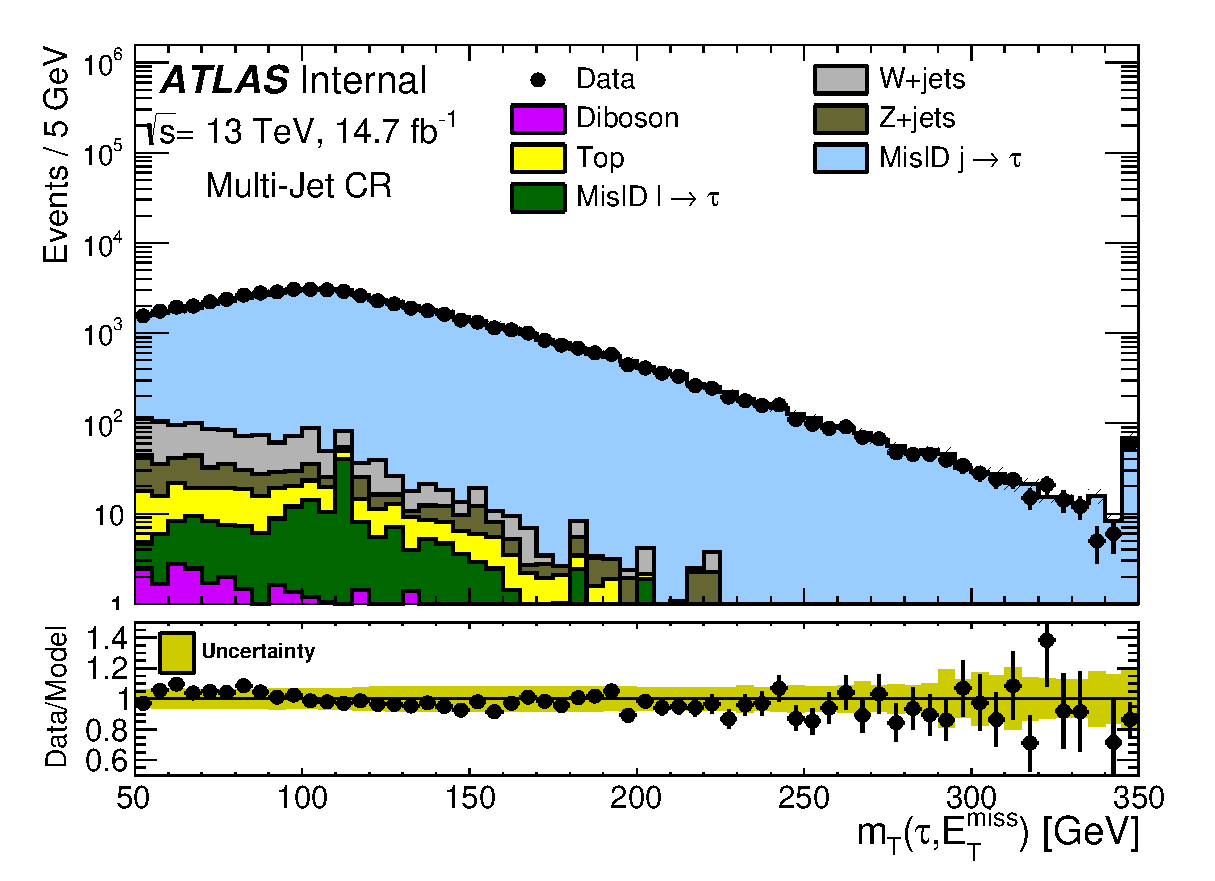
\includegraphics[width=\textwidth]{figures/DDQCD15_QCD_MT.eps}
\caption{}
\end{subfigure} % 
\begin{subfigure}{0.5\textwidth}
   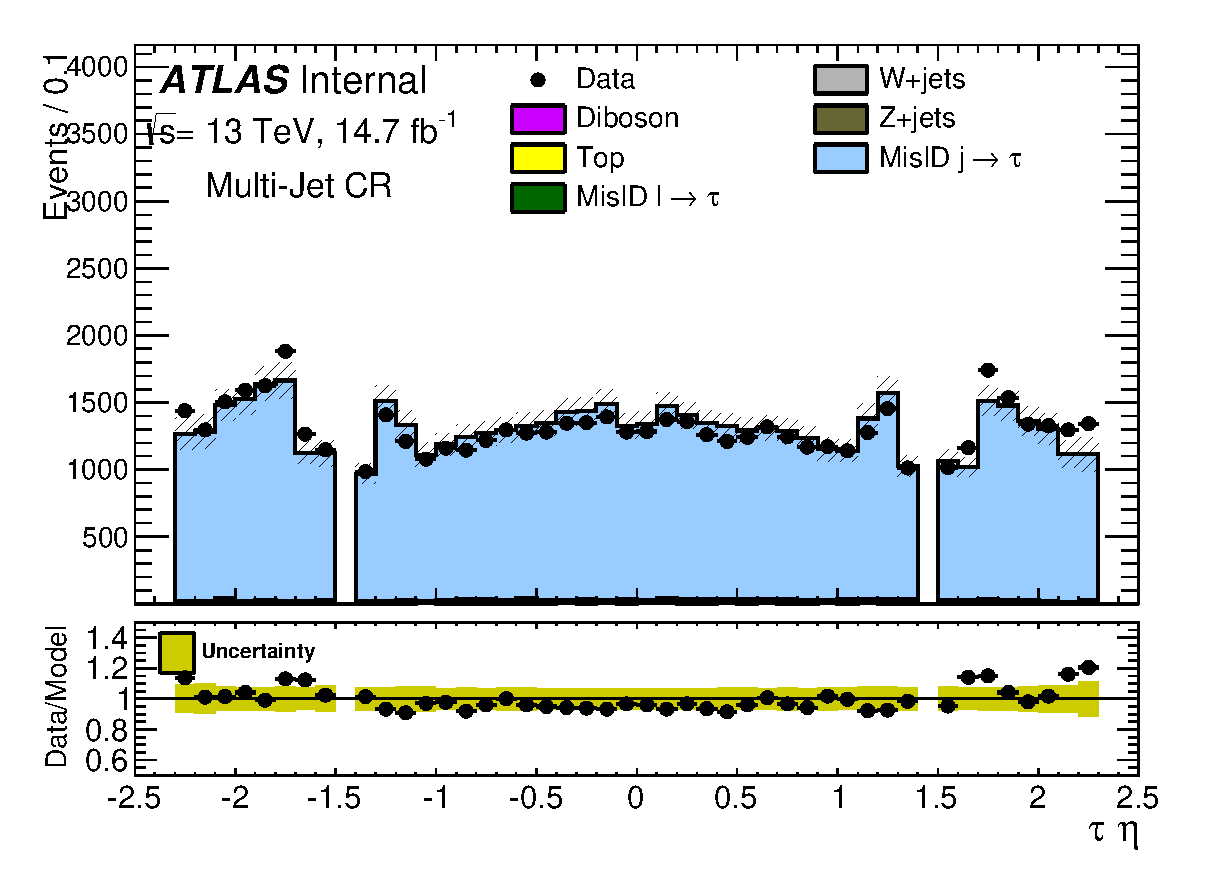
\includegraphics[width=\textwidth]{figures/DDQCD15_QCD_taueta.eps}
\caption{}
\end{subfigure}
\caption{\FF\ closure plots in the multi-jet measurement control region}
\label{fig:clMultiJ}
\end{figure}

\par To evaluate the \FF\ robustness to change in jet composition, two 
control regions were used. As alreadly mentioned, the \Wjets\ region is dominated by jets initiated 
by light-flavored quarks. Contrastingly, a region rich in \ttbar\ events is dominated by 
jets initiated by heavy-flavored quarks. These two regions were used to evaluate the impact of 
heavy versus light-flavored quarks on \FF\ modelling, and vice-versa. Figure~\ref{fig:clWjets} and Figure~\ref{fig:clTTBar}
show the estimated $j\to\tau$ background using the \FF\ method  in the $\Wjets$ and $\ttbar$ control 
regions respectively. The modelling in the $\Wjets$ control region is good, while the modelling in the 
$\ttbar$ control region shows an overall event underestimation. The statistical uncertainties in the 
$\ttbar$ control region are larger, indicating that the observed underestimation may be 
statistical in nature.   

\begin{figure}[!h]
\begin{subfigure}{0.5\textwidth}
   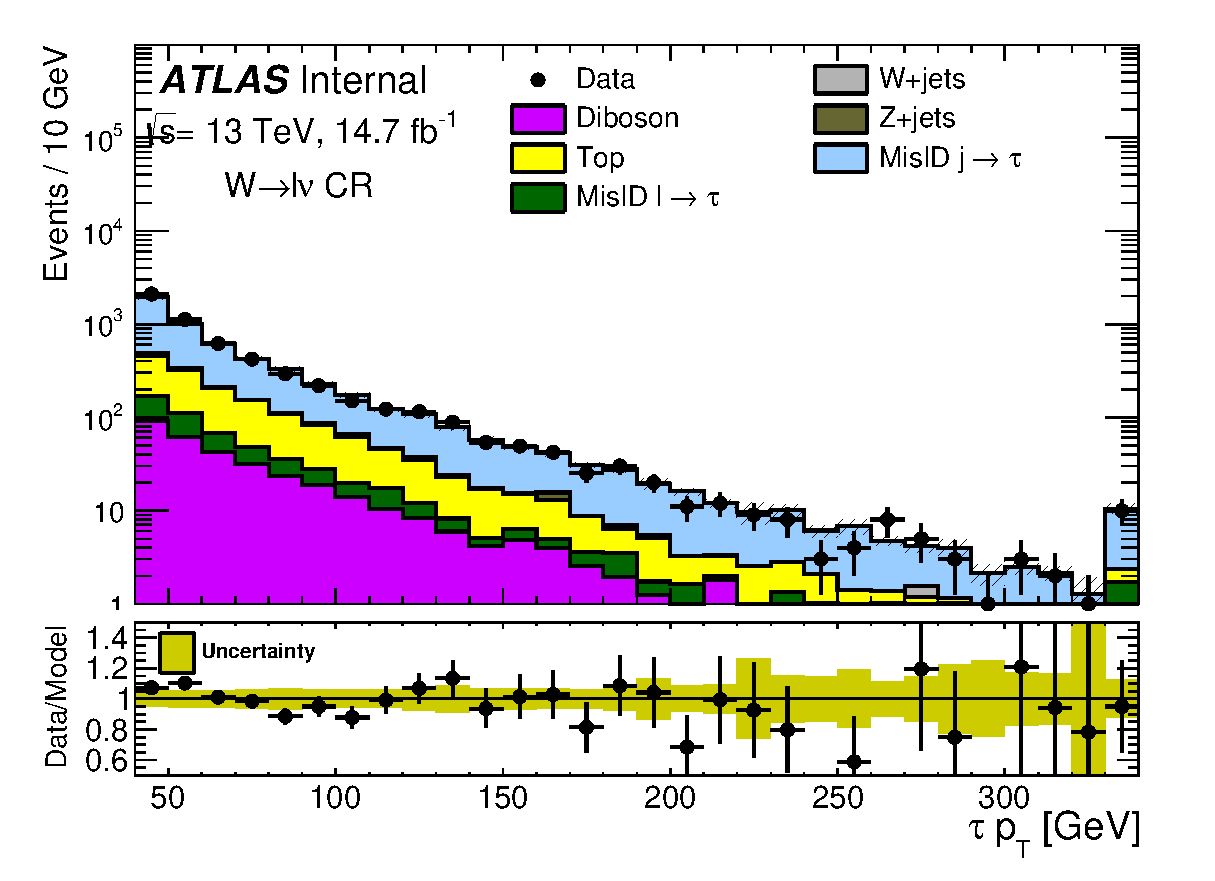
\includegraphics[width=\textwidth]{figures/DDQCD15_FFWCR_taupt_log.eps}
\caption{}
\end{subfigure} % 
\begin{subfigure}{0.5\textwidth}
   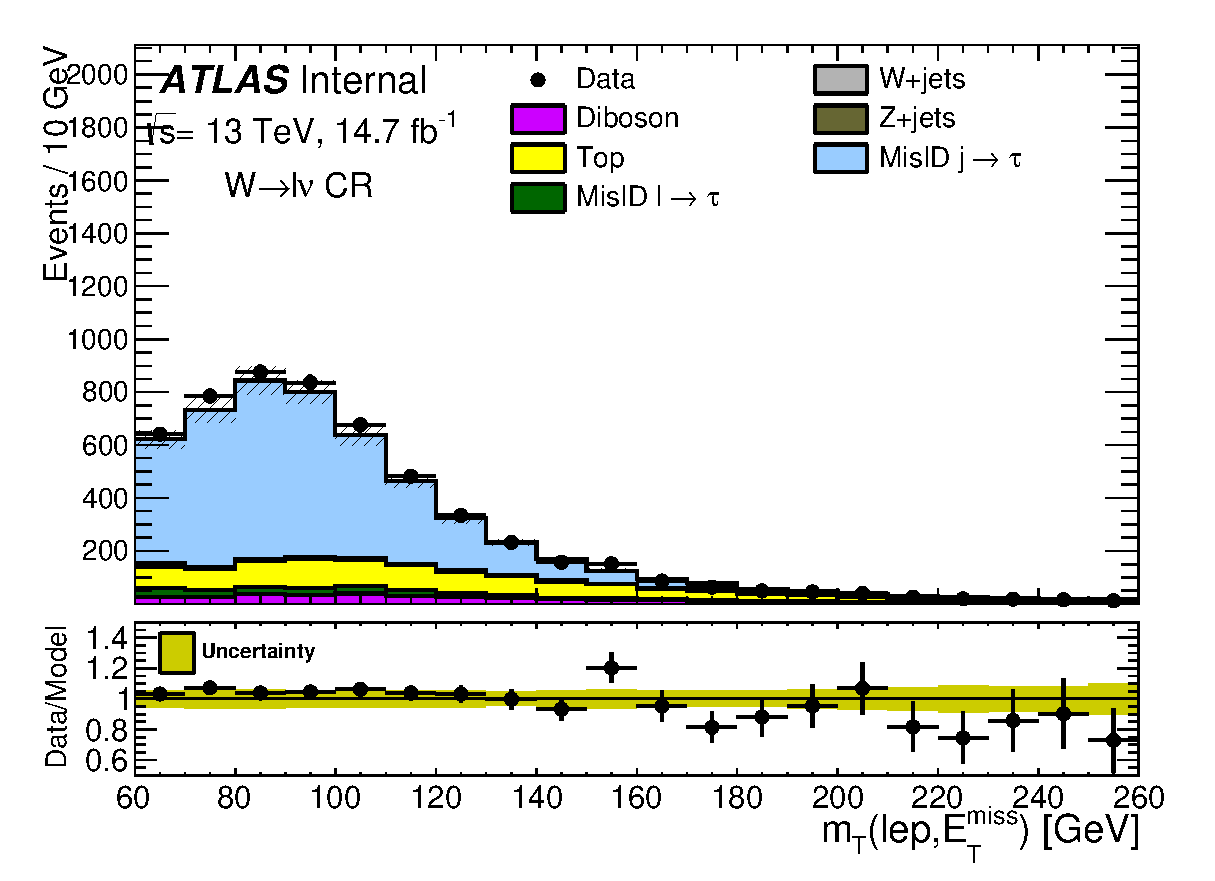
\includegraphics[width=\textwidth]{figures/DDQCD15_FFWCR_WlepMT.eps}
\caption{}
\end{subfigure}
\caption{\FF\ closure plots in the \Wjets\ control region}
\label{fig:clWjets}
\end{figure}

\begin{figure}[!h]
\begin{subfigure}{0.5\textwidth}
   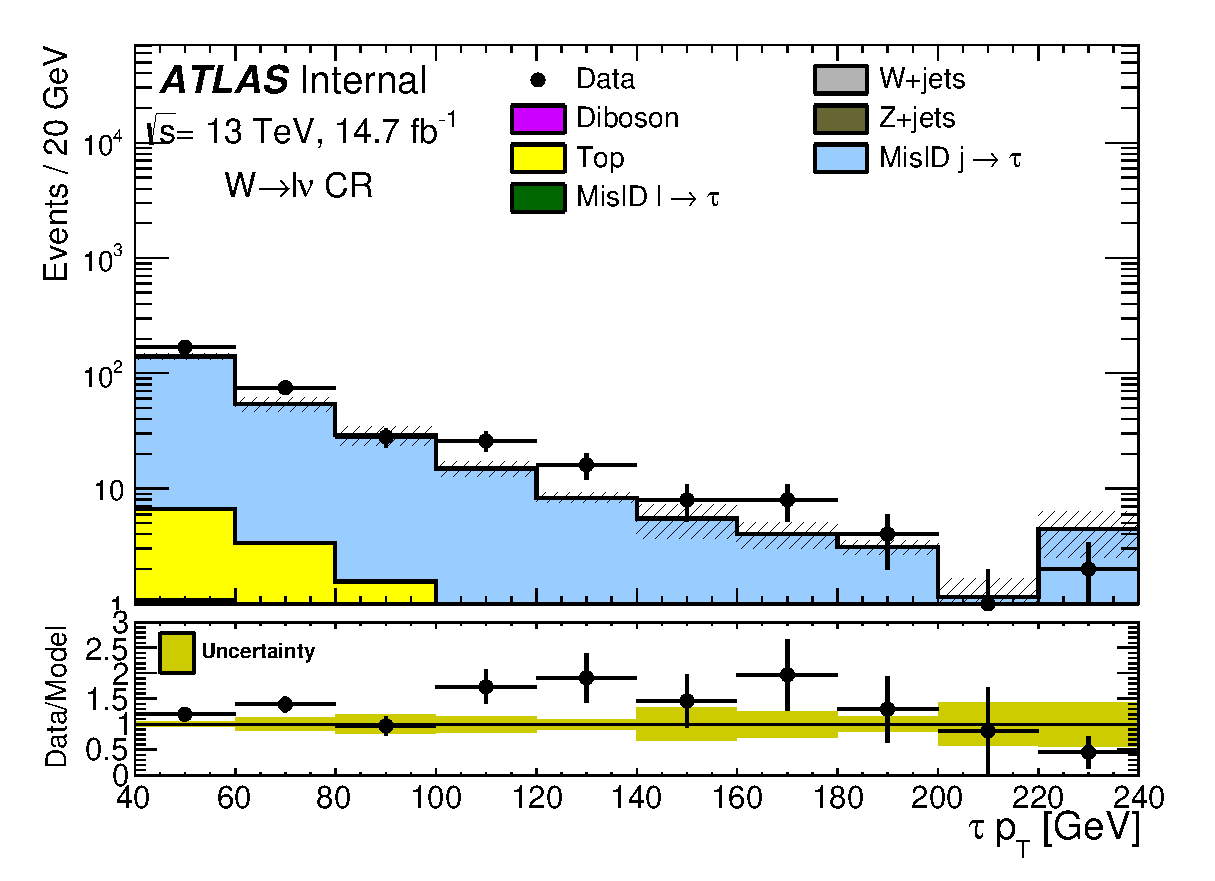
\includegraphics[width=\textwidth]{figures/DDQCD15_FFttll_taupt_log.eps}
\caption{}
\end{subfigure} % 
\begin{subfigure}{0.5\textwidth}
   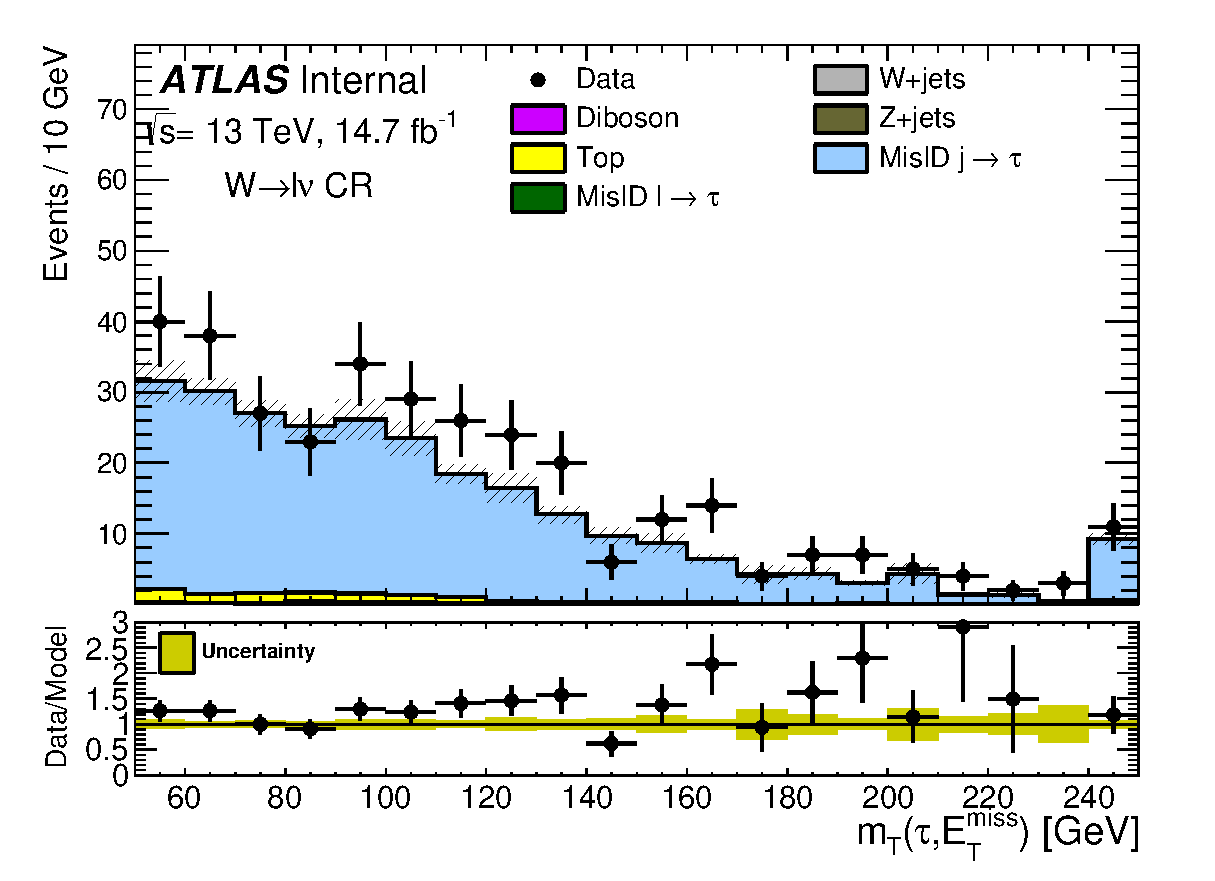
\includegraphics[width=\textwidth]{figures/DDQCD15_FFttll_MT.eps}
\caption{}
\end{subfigure}
\caption{\FF\ closure plots in the \ttbar\ control region}
\label{fig:clTTBar}
\end{figure}


\subsection{True $\tauvis$ backgrounds}
\label{sec:truetau}
\par True $\tauvis$ backgrounds are estimated from Monte Carlo simulation. 
Such backgrounds expected in the signal region are shown in Figures~\ref{fig:preselectA} and~\ref{fig:preselectB}.
Top and $\Wjets$ processes are expected to dominate these backgrounds, while a few $\Zboson+$jets and $VV$ 
events are also expected to contaminate the signal region.

\par \ttbar\ may be mis-classified as signal  
 when one of the top quarks decays leptonically as 

\begin{equation}
\begin{aligned}
t\to \Wplus b\to\tau\nu_\tau  &  & \text{and the other as,} \\
t\to \Wplus b\to qqb. &  &
\end{aligned}
\label{eq:ttBarDc}
\end{equation}

In this topology, the $\nu_\tau$  is reconstructed as $\met$ and the $\tau$ as $\tauvis$; the three quarks from the other 
top decay may be reconstructed as jets, one of which may be $b-$tagged.  
The $\mT(\tau,\nu_\tau)$, is usually 
low in this topology because the $\tauvis$ and \met\ are expected to be aligned in $\phi$. 
The secondary method of \ttbar signal contamination is when both top quarks decay 
leptonically and one of the leptons is not identified or reconstructed. In this case \mT\ is expected to be 
high because the \met\ is a reconstruction of two $\nu_\tau$.
A single top can get mis-classified as signal when the top quark decays leptonically, and the 
associated quarks are reconstructed as jets. Note that only the $Wt-$channel has multiple jets in the 
leading order calculation. So, contribution of single top to the signal region is relatively smaller than that 
of \ttbar. 

\par $\Wjets$ events enter the signal region when the $\Wplus$ decays to a $\tau$ lepton and a $\nu_\tau$. 
Since the signal region requires at least 3 jets in the event, \Wjets\ only enters the signal 
region if it has 3 or more associated jets.

\par Since \ttbar\ and \Wjets\ are the most dominant backgrouns processes in the signal region, 
dedicated control regions in data are devised to assess their modelling in simulation.   
For this assessment to be extrapolated to the signal region, these control regions 
are designed to be as close as possible to it. They are also designed to have as few signal events 
as possible to reduce bias.
 
\par The \ttbar\ control region differs from the signal region in that 2 or more $b-$tagged jets 
and $\mT<100$~\GeV\ are required. The $b-$tagged jets requirement is justifiable from Equation~\ref{eq:ttBarDc}. 
 The low $\mT$ selection is to maximize \ttbar\ events in which 
one of the top quarks decays to a $\tau$ lepton, while refraining from the high \mT\ region that is 
part of the signal region. With this selection criteria the \ttbar\ control region has a small 
overlap with the signal region, but the expected signal contamination is about one order of 
magnitude smaller than the expected fraction of \cHtaunu\ events in the signal region. Kinematic 
distributions in this region are shown in Figure~\ref{fig:ttBarCR}. 

\par The \Wjets\ control region differs from the signal region in that it requires events 
to have no $b-$tagged jets and have $mT<100$~\GeV. This region is orthogonal to the signal 
region, and yet close to the signal region in phase space. Kinematic variables are shown in 
Figure~\ref{fig:wjetsCR}.  

\begin{figure}[!h]
\begin{subfigure}{0.5\textwidth}
   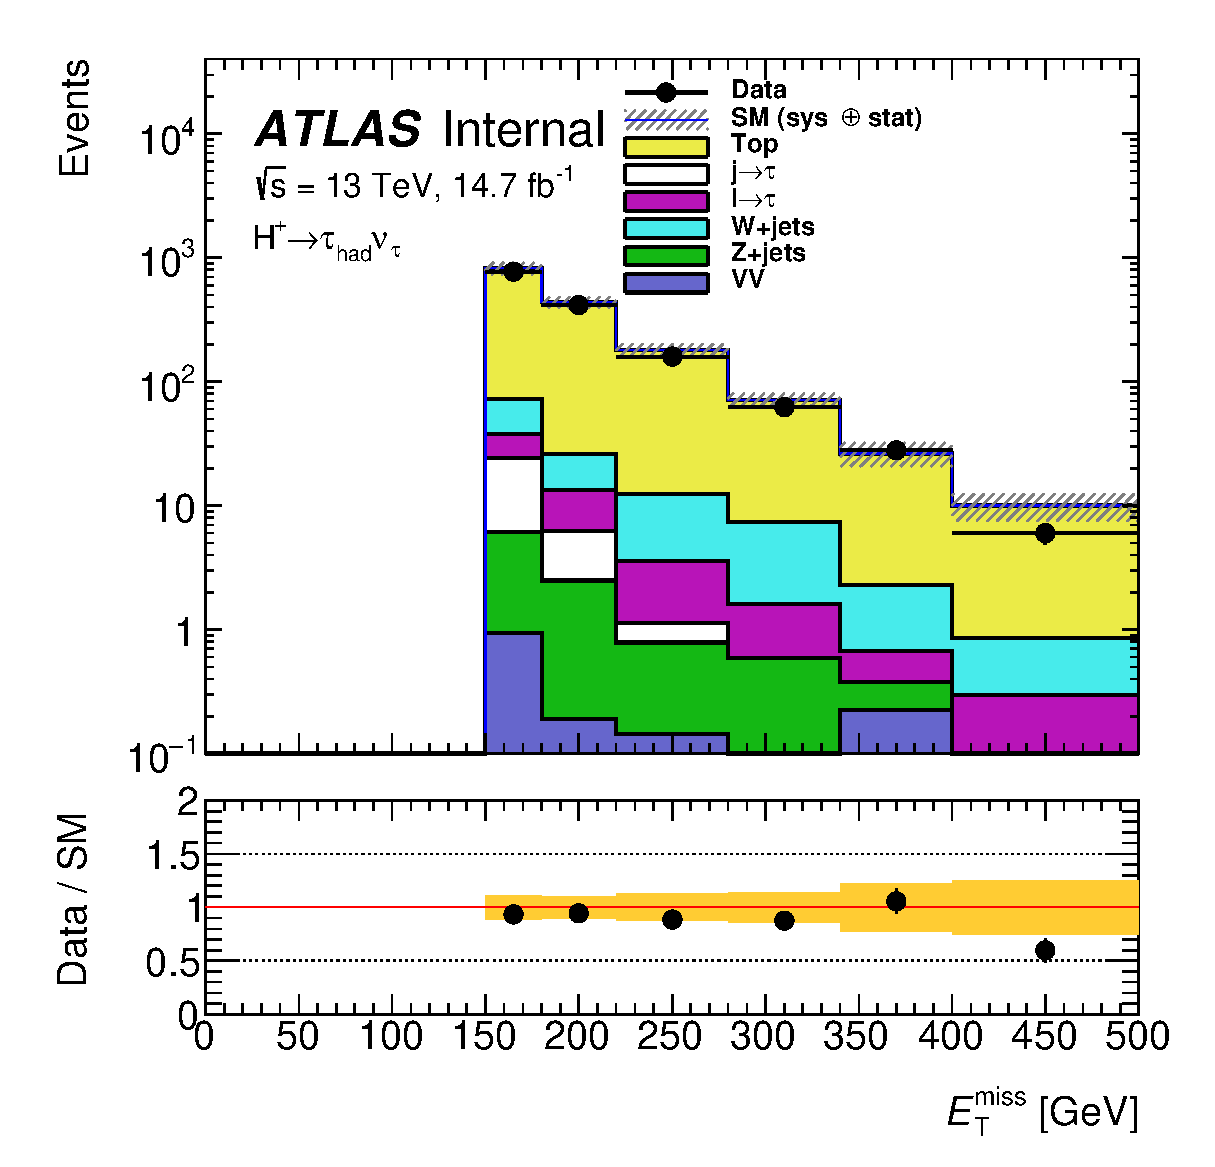
\includegraphics[width=\textwidth]{figures/met_TTBar.eps}
\caption{\met}
\end{subfigure} % 
\begin{subfigure}{0.5\textwidth}
   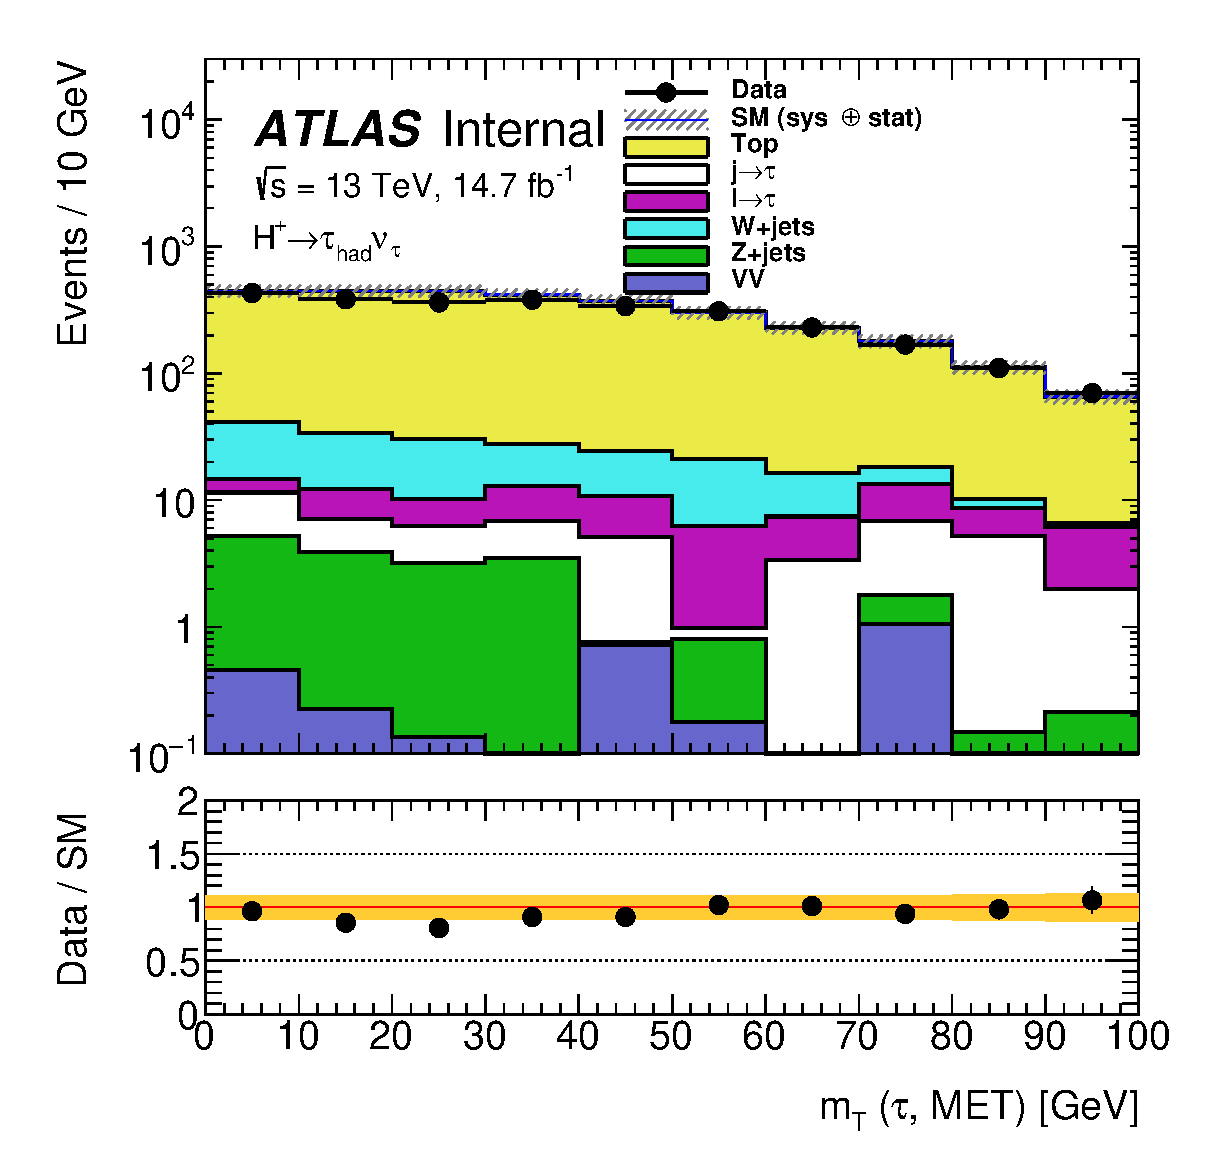
\includegraphics[width=\textwidth]{figures/mT_TTBar.eps}
\caption{\mT}
\end{subfigure}
\begin{subfigure}{0.5\textwidth}
   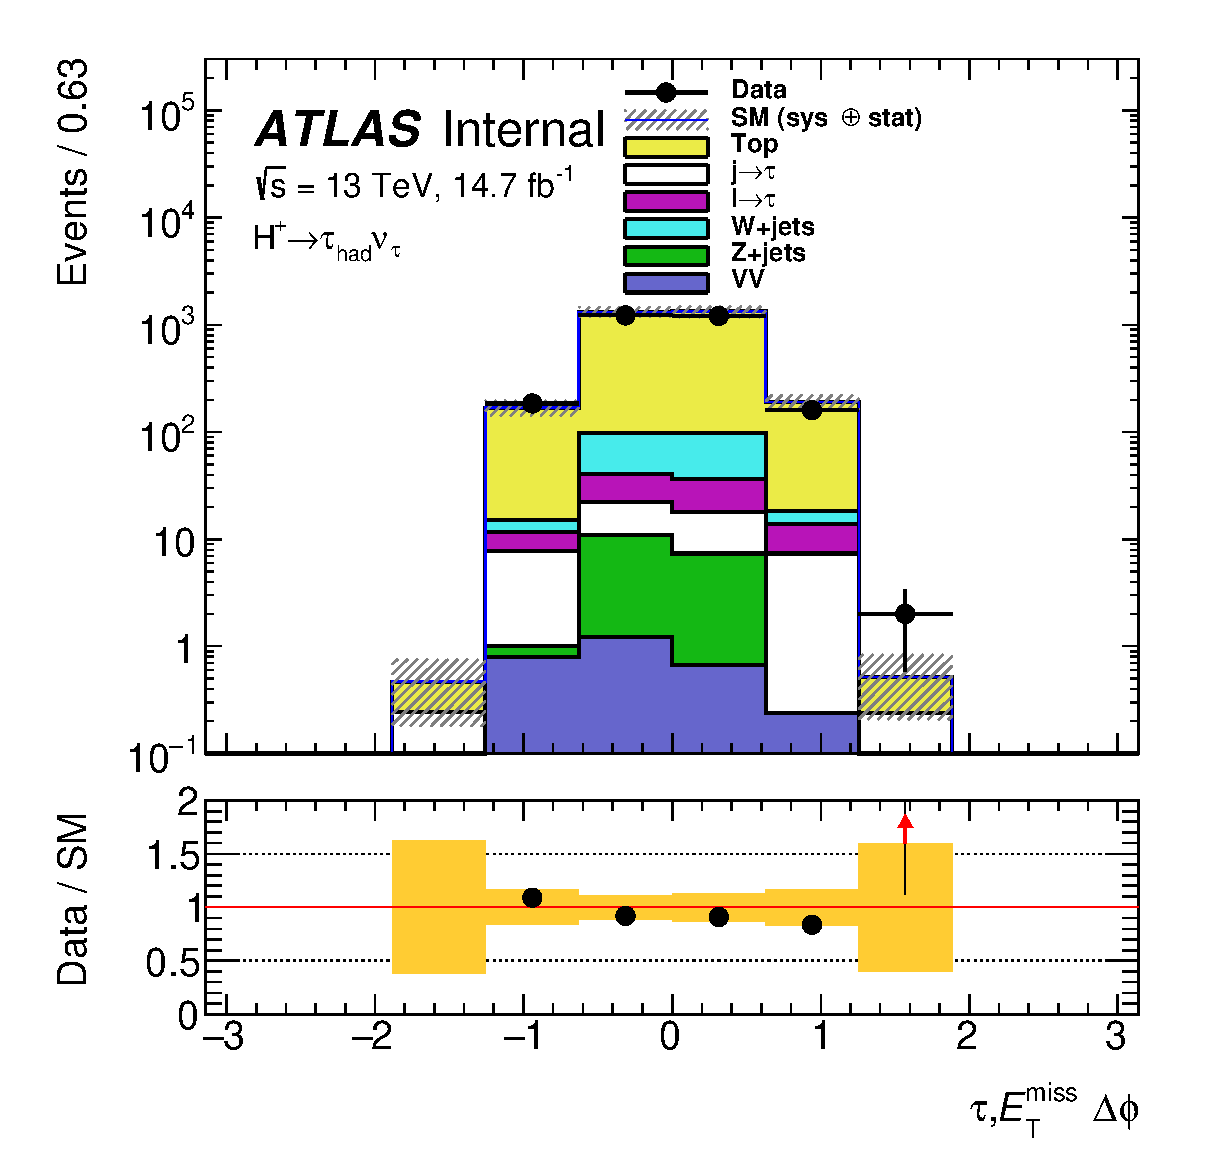
\includegraphics[width=\textwidth]{figures/taumetphi_TTBar.eps}
\caption{}
\end{subfigure} % 
\begin{subfigure}{0.5\textwidth}
   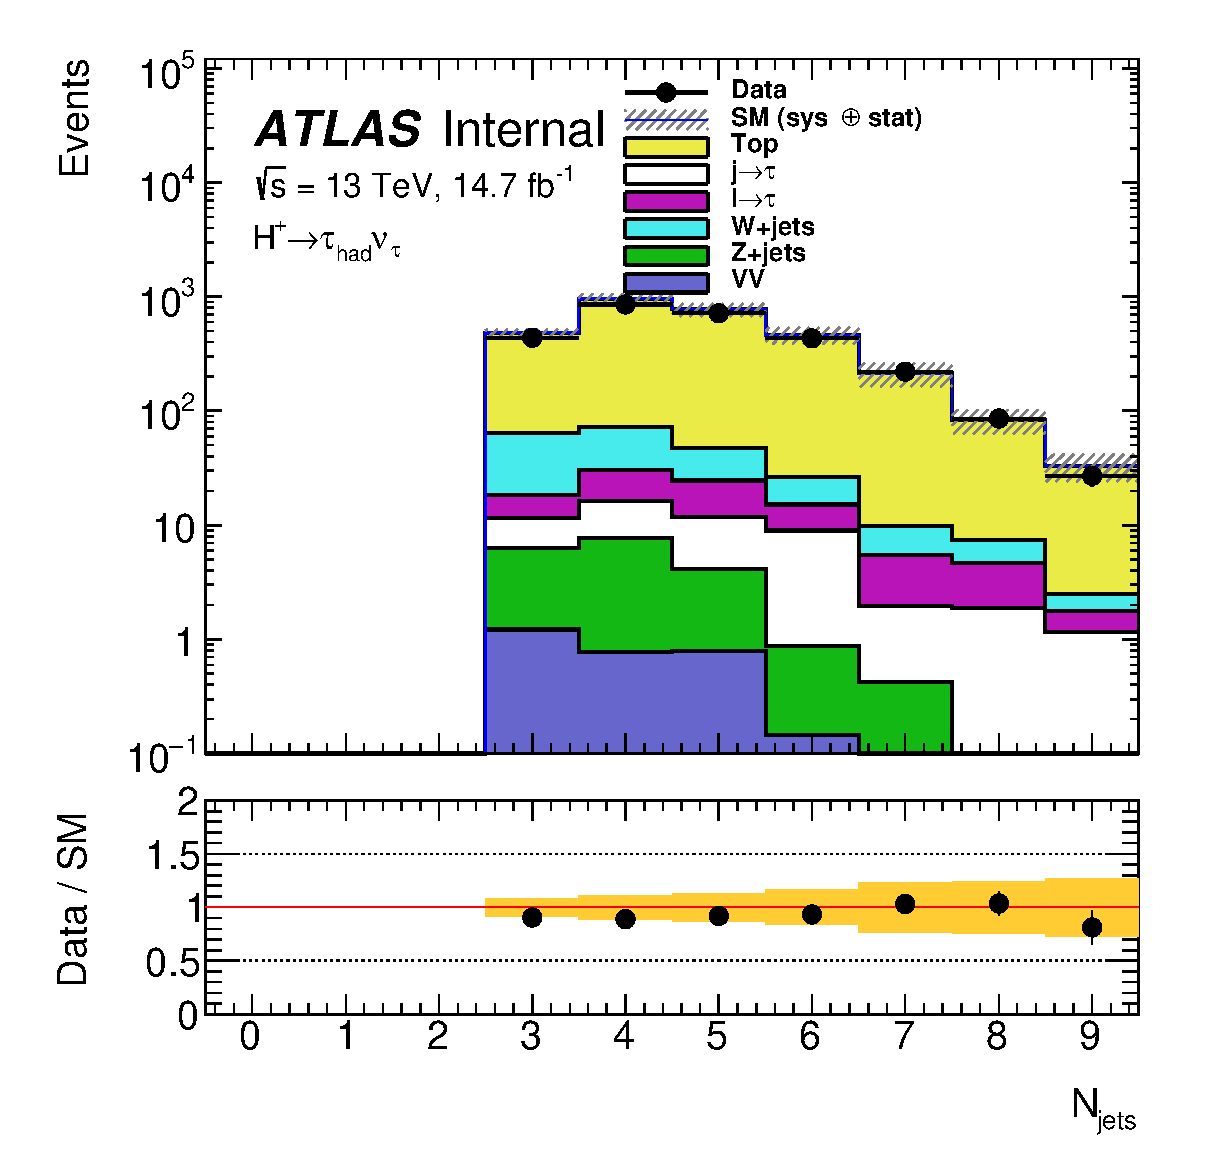
\includegraphics[width=\textwidth]{figures/nJets_TTBar.eps}
\caption{Number of jets}
\end{subfigure}
\caption{Plots showing kinematic distributions in the \ttbar\ control region}
\label{fig:ttBarCR}
\end{figure}

\begin{figure}[!h]
\begin{subfigure}{0.5\textwidth}
   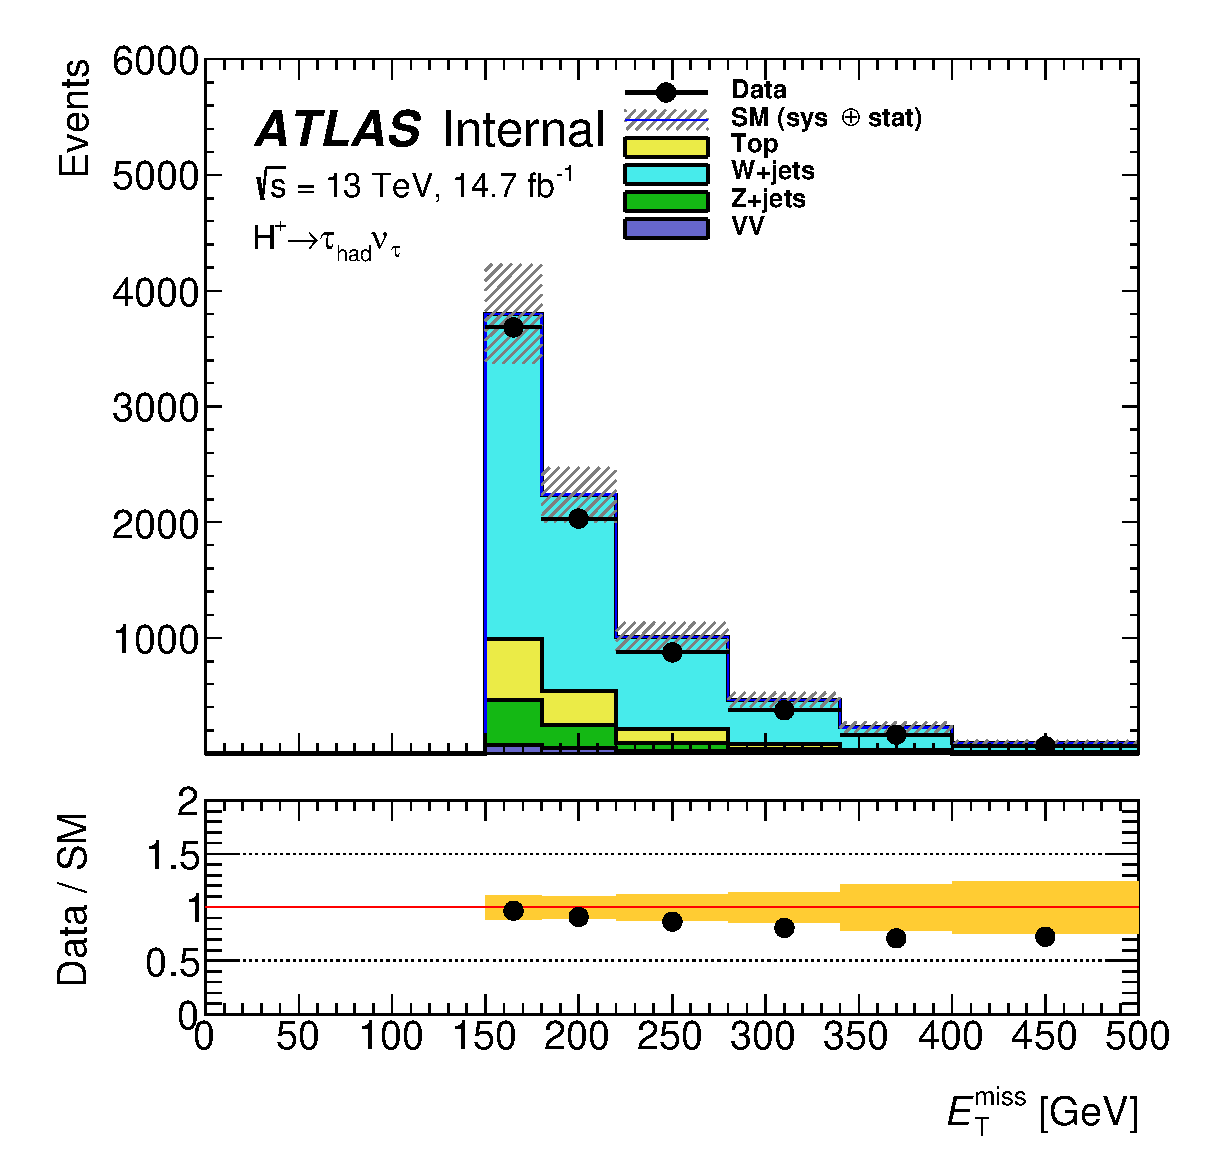
\includegraphics[width=\textwidth]{figures/met_Wjets.eps}
\caption{\met}
\end{subfigure} % 
\begin{subfigure}{0.5\textwidth}
   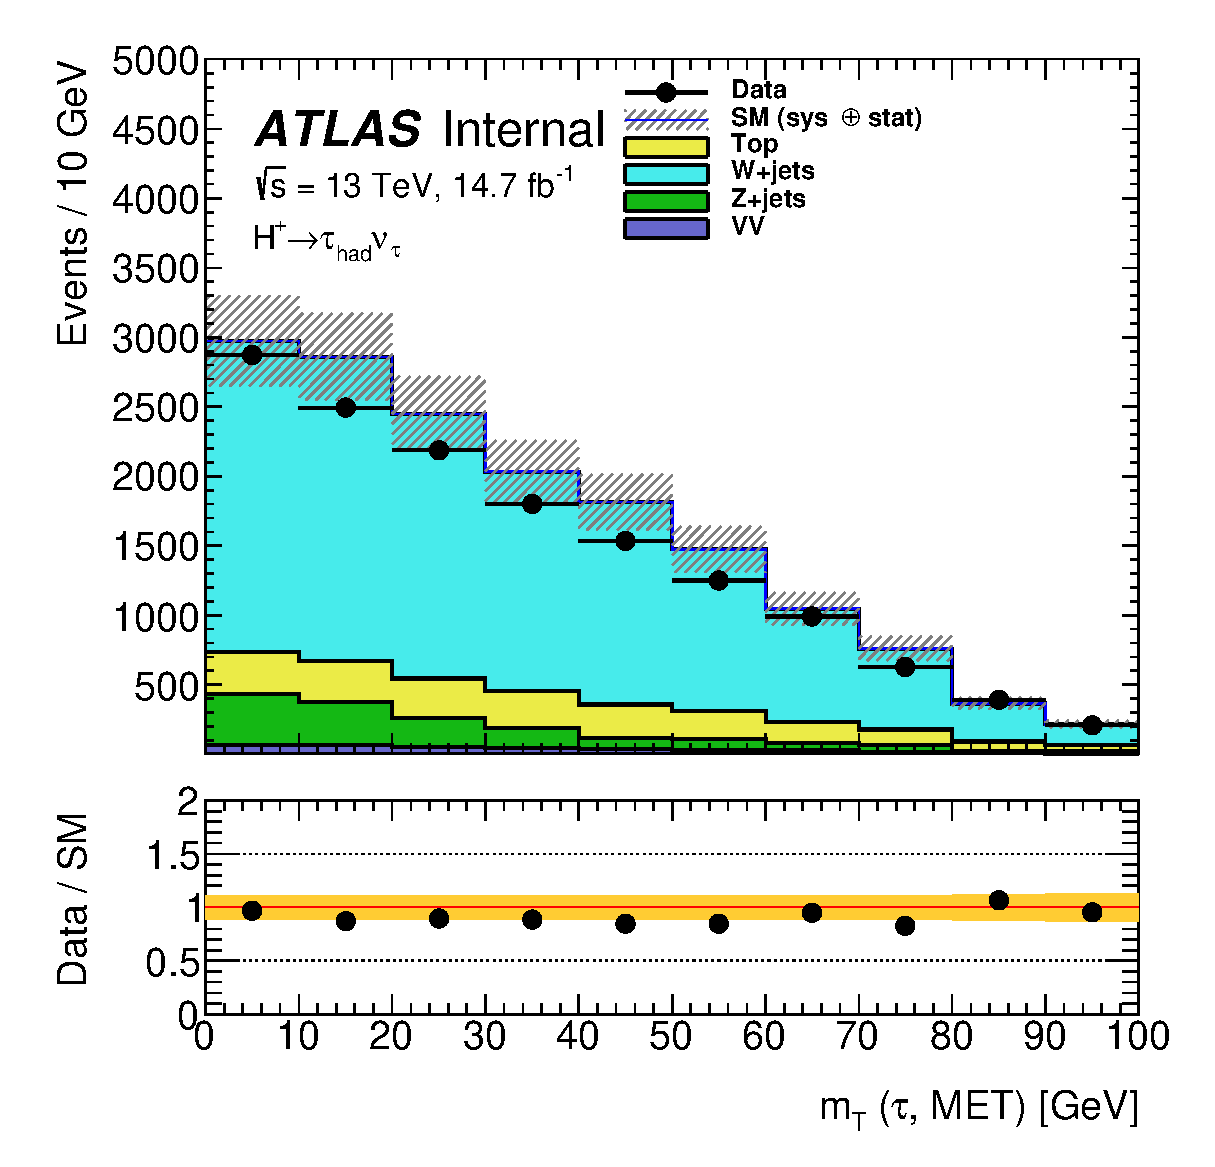
\includegraphics[width=\textwidth]{figures/mT_Wjets.eps}
\caption{\mT}
\end{subfigure}
\begin{subfigure}{0.5\textwidth}
   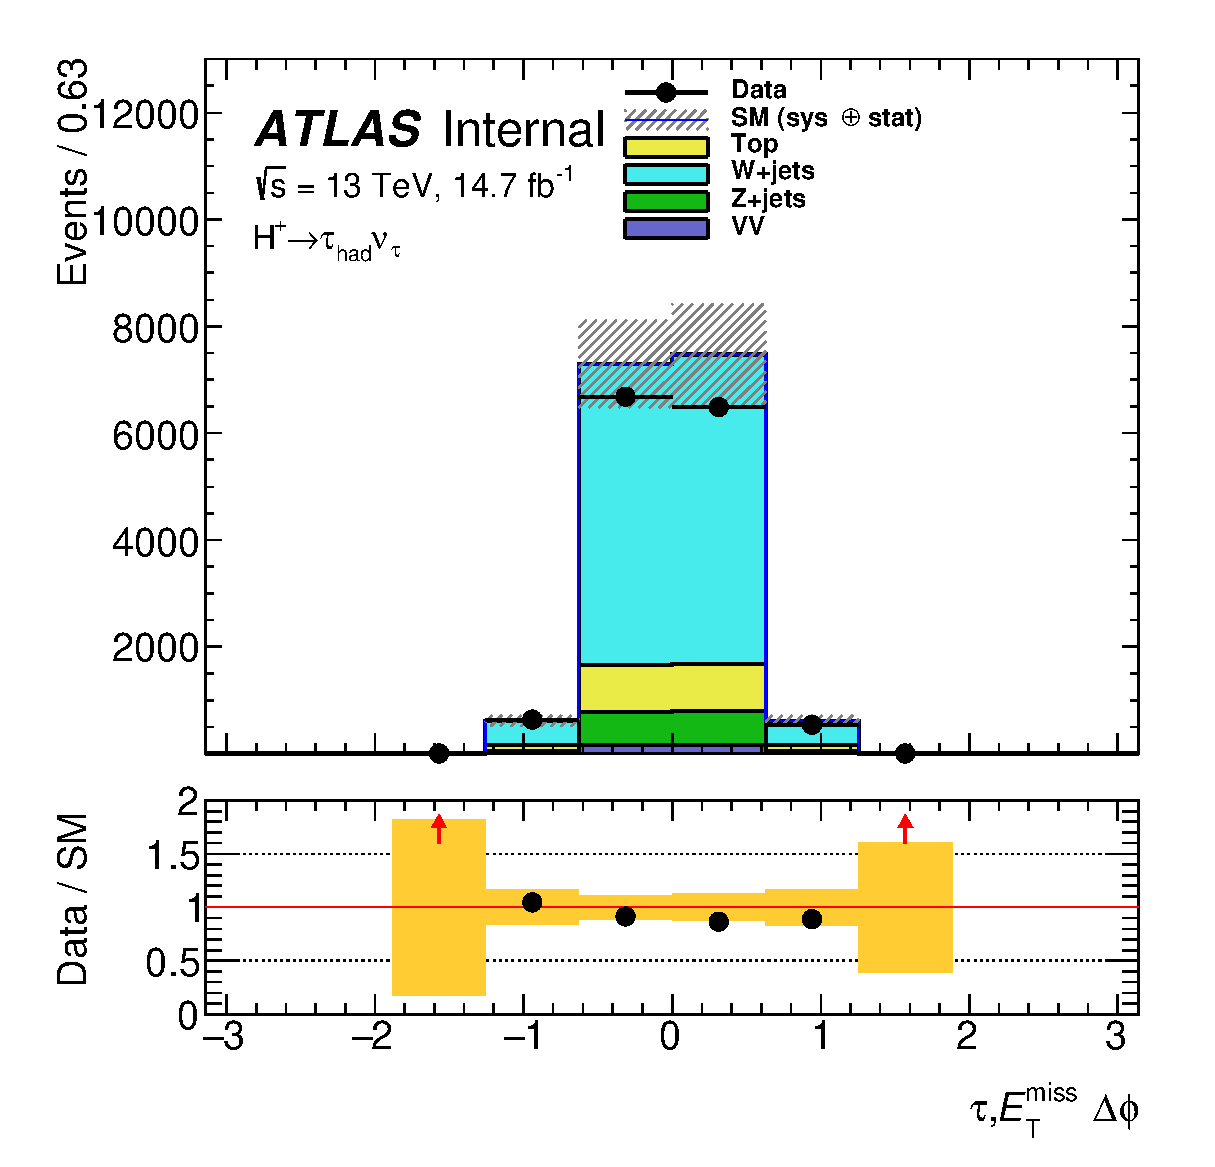
\includegraphics[width=\textwidth]{figures/taumetphi_Wjets.eps}
\caption{}
\end{subfigure} % 
\begin{subfigure}{0.5\textwidth}
   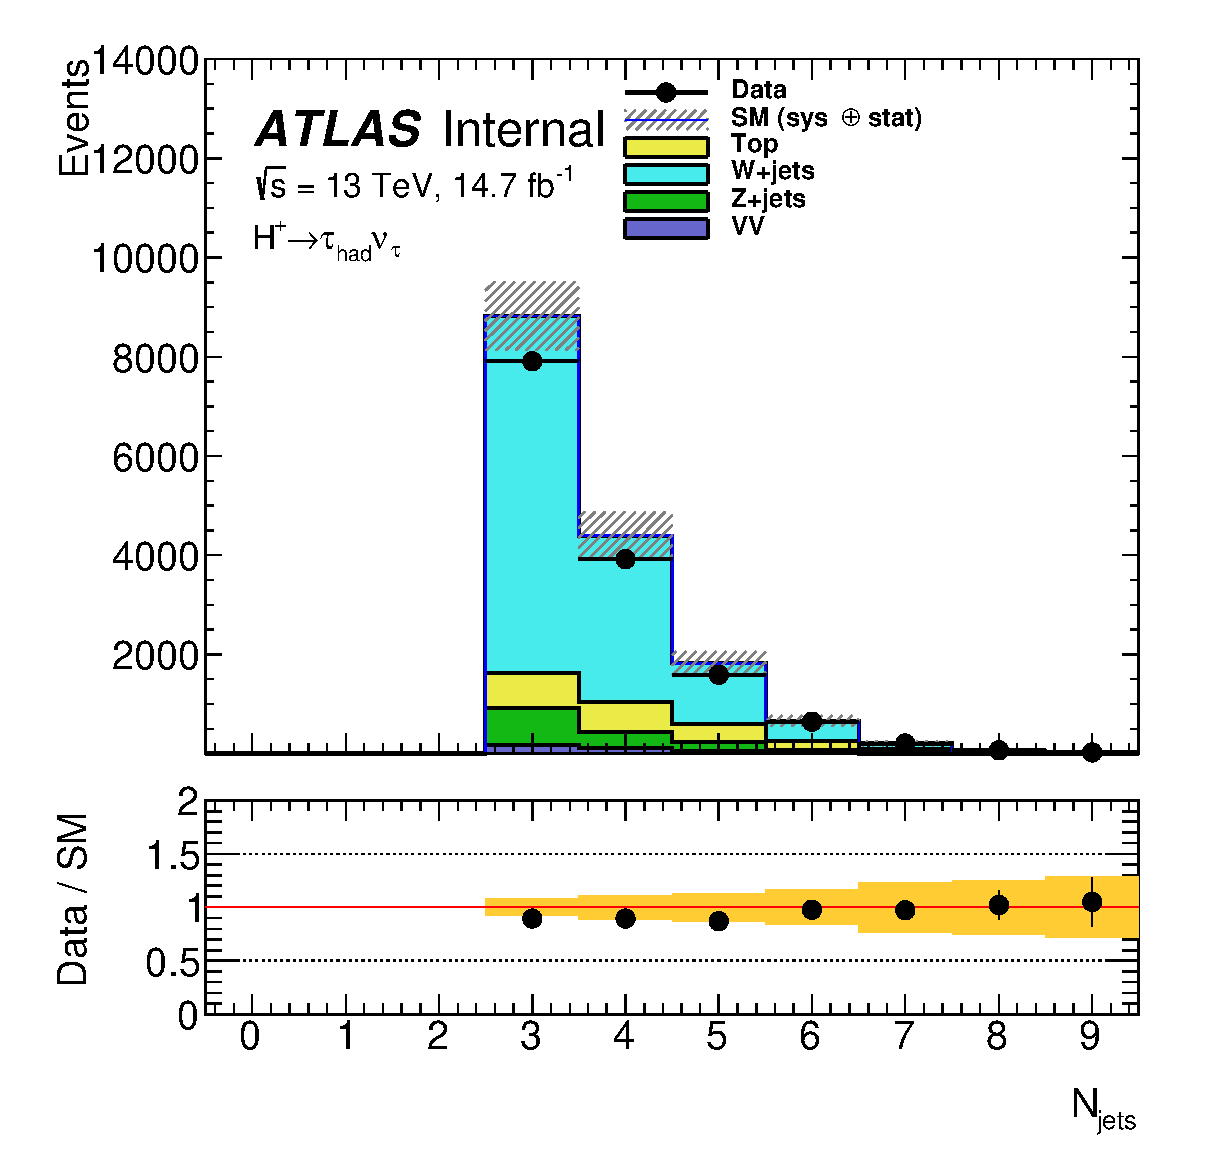
\includegraphics[width=\textwidth]{figures/nJets_Wjets.eps}
\caption{Number of jets}
\end{subfigure}
\caption{Plots showing kinematic distributions in the \Wjets\ control region}
\label{fig:wjetsCR}
\end{figure}

